\chapter{MINERvA experiment}
\label{ch:minerva}

\begin{tikzpicture}[remember picture,overlay]
    \node[anchor=east,inner sep=0pt] at (current page text area.east|-0,5cm) {
\includegraphics[height=4cm]{03minerva/figures/minerva_pride.jpeg}};
\end{tikzpicture}
    
\vspace{-30pt}
MINERvA (Main Injector Neutrino ExpeRiment to study $\nu$--A interactions) was an experiment specifically designed to perform self-contained studies of nuclear dependence in (anti)neutrino scattering. Operational from 2009 until the conclusion of its physics run in 2019, the experiment was situated in the MINOS near detector hall at Fermi National Accelerator Laboratory (Fermilab). At its core was the MINERvA detector, which was exposed to muon (anti)neutrinos from the high-intensity Neutrinos at the Main Injection (NuMI) beam. An integral part of the experiment involved using the data from the MINOS (Main Injector Neutrino Oscillation Search) near detector, utilized as a (anti)muon spectrometer, to constrain the momenta of (anti)muons generated by charged-current (anti)neutrino interactions within the MINERvA detector. This chapter delves into these three components of the experiment enabling the high-precision measurements of (anti)neutrino interactions, with a particular focus on the aspects relevant to the measurement presented in this work.

\vspace{-5pt}
\section{NuMI beamline}\label{sec:NuMI}
% numi beam description 2-16: https://www.sciencedirect.com/science/article/pii/S016890021501027X
% Neutrino flux prediction thesis: Aliaga: https://web.archive.org/web/20190427031702id_/https://scholarworks.wm.edu/cgi/viewcontent.cgi?article=1036&context=etd
% Amit bashyal thesis (antineutrino measurement): https://lss.fnal.gov/archive/thesis/2000/fermilab-thesis-2021-03.pdf

The Neutrinos at the Main Injector (NuMI) beamline \cite{numiTDR_osti_1156372, numi2016_ADAMSON2016279} is a conventional accelerator neu\-trino source originally constructed to supply muon (anti)neutrinos for the long-baseline neutrino oscillation experiment MINOS \cite{MINOS:1998kez, MINOS_PhysRevLett.97.191801}. It was later upgraded to provide a higher-intensity beam for its successor, NOvA \cite{NOVA_2005nova}. The (anti)neutrinos are produced via decays of charged pions and kaons, which, in turn, are created from protons striking a graphite target. A~schematic of the NuMI beamline starting from the graphite target is depicted in Figure~\ref{fig:numi}. The MINERvA experiment spanned both the MINOS and NOvA configuration of the NuMI beamline, with peak (anti)neutrino energies of $\sim$3~GeV and $\sim$6~GeV, respectively. These are referred to as the low energy~(LE) and medium energy~(ME) regimes. The measurement described in this work utilises the ME~antineutrino dataset exclusively, which is reflected in the description of the NuMI configuration. Both the instrumentation of the NuMI beamline and the simulation prediction of the NuMI flux are discussed.

\begin{figure}[t!] 
    \vspace{-5pt}
    \centering
    {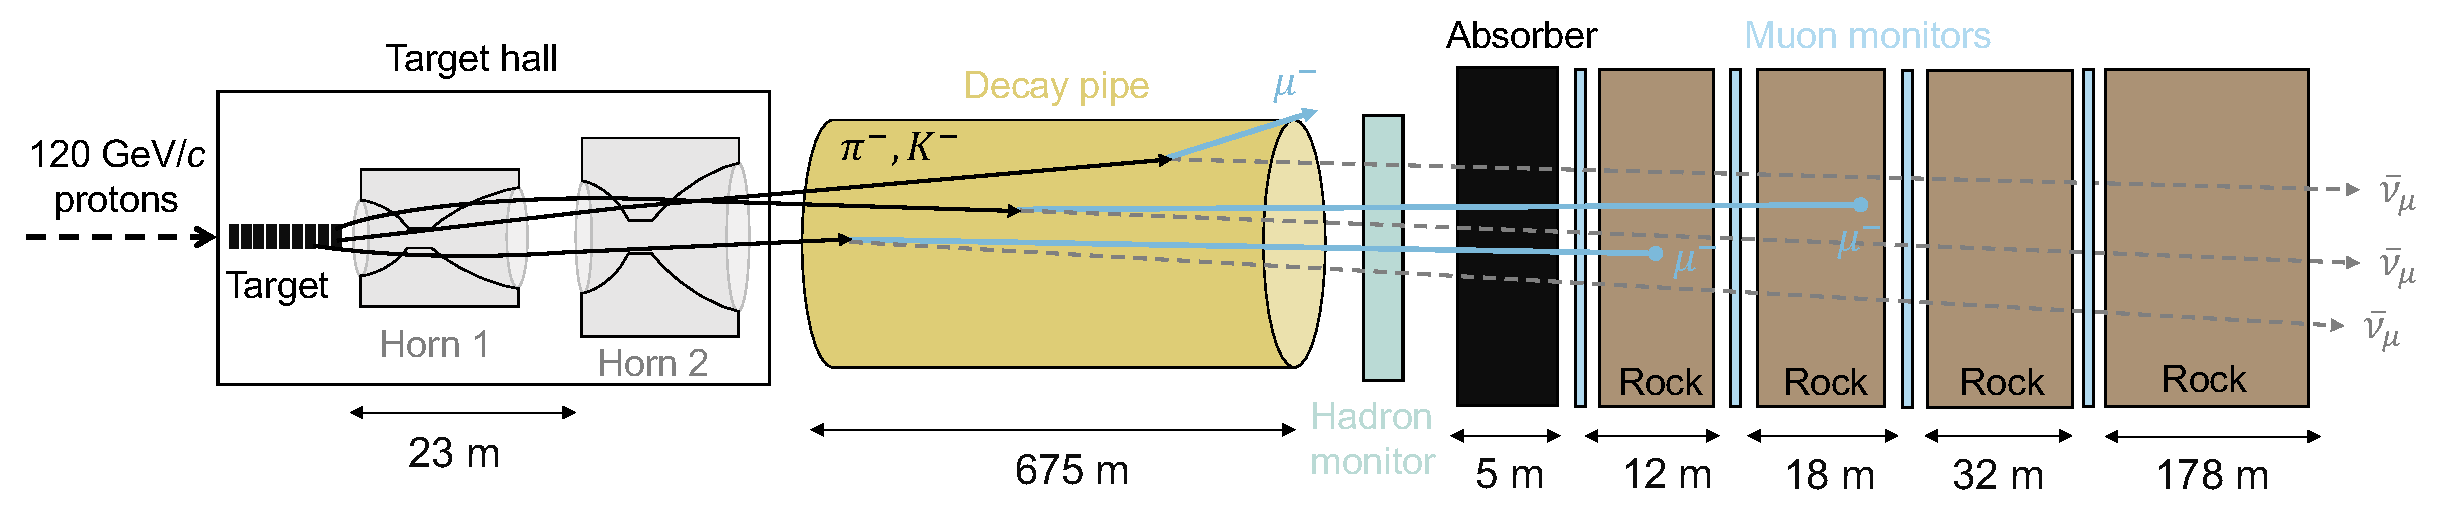
\includegraphics[width=1.\textwidth]{03minerva/figures/numiBeamline.pdf}}%
    \caption{Schematic illustrating the components of the NuMI beamline at Fermilab in the medium energy reverse horn current configuration, drawn based on the information provided in Refs.\cite{numi2016_ADAMSON2016279,TiceThesis2014}. }
    \label{fig:numi}
\end{figure}

\subsection{Instrumentation}

The NuMI beamline hardware and operations are in detail described in Ref.~\cite{numi2016_ADAMSON2016279}. First, protons from hydrogen ions undergo incremental acceleration in Fermilab's proton accelerator complex \cite{fnalAccelerator_Convery:2018ltx}, including the linear accelerator (Linac) and Booster synchrotron, ultimately reaching the final beam energy of 120~GeV in the Main Injector synchrotron accelerator.~Subsequently, these protons are extracted and directed onto the~graphite target in approximately 10~$\mu$s long windows, referred to as spills. Upon the extraction from the MI, the proton beam is also bent 3.343$^\circ$ (58.87~mrad) downwards towards the MINOS far detector in Minnesota.

Compared to the LE era, the beam intensity was increased from 400 kW to more than 700 kW in the ME era by placing more protons in the same spill and reducing the spill cycle time to 1.33~seconds from the original 2.2 seconds. The ME configuration delivered around 4.9$\times 10^{13}$ protons on target~(POT)\footnote{The number of protons on target (POT) is a metric used to characterise the integrated luminosity of the (anti)neutrino beam.} during each spill, resulting in the total data exposure of $1.12 \times 10^{21}$~POT recorded by MINERvA and used for this measurement.  The total number of POT collected by MINERvA over its physics run both in the LE and ME era is summarised in Table \ref{table:pot}.

\begin{table}[t!]
    \vspace{-10pt}
    \centering
    \begin{tabular}{c c c}
    \hline \\ [-1.5 ex]
    \multirow[c]{2}{*}{Regime}& \multicolumn{2}{c}{Mode (POT)} \\
    & Neutrino-dominated & Antineutrino-dominated\\ [0.5ex] % inserts table %heading
    \hline
    \hline \\[-1.8ex]
    Low (LE) $\sim$3~GeV & $4.0\times 10^{20}$ & $1.7 \times 10^{20}$ \\ 
    Medium (ME) $\sim$6~GeV & $10.6 \times 10^{20}$ & $11.2 \times 10^{20}$ \\
    \hline
    \end{tabular}

    \caption{The number of protons on target recorded by MINERvA in the low and medium energy regime for both neutrino and antineutrino-dominated beams.}
    \label{table:pot}
\end{table}


% To talk about the numi beam + angle
%https://lss.fnal.gov/archive/2015/pub/fermilab-pub-15-253-ad-fess-nd.pdf
% Upgrade to fermilab beam line for NOvA ,where I got the numbr  for the parameters
%https://ieeexplore.ieee.org/stamp/stamp.jsp?tp=&arnumber=4440873

Prior to reaching the graphite target, the proton beam is collimated by passing through a hole in the so-called baffle---a graphite-aluminum tube designed to partially degrade mis-steered beams to protect other components of the beamline. The proton beam size is about $\sim$1~mm upon impinging onto the 1.2~metres long (about 2.5 proton interaction lengths) graphite target. The target is made out of 50 narrow fins to dissipate heat and reduce the probability of reinteraction of produced hadrons, which are mounted on steel pipes providing water cooling and contained within a helium-filled vessel.

The final state particles produced by the proton beam hitting the target, mostly pions and kaons, are charge-sign selected and focused in a forward direction by two 3~metres long parabolic magnetic horns made of aluminum.~The choice of the horn current direction, whether it is forward horn current (FHC) or reverse horn current (RHC), determines the selection of positive or negative charged hadrons, ultimately resulting in a neutrino or antineutrino-dominated beam, respectively.~The RHC configuration is shown in Figure~\ref{fig:horns}. The horns increase the hadron flux in the desired energy range and provide flexibility in choosing that energy based on their configuration. The ME~spectra with the (anti)neutrino energy peak of $\sim$6~GeV was achieved by increasing the distance between the target and the first horn, and the first horn and the second horn compared to the LE configuration.\enlargethispage{2\baselineskip}~During the antineutrino-dominated runs used in this measurement, the magnetic field was generated by a~$-200$~kA electric horn current into the horns. 

\begin{figure}[t!] 
    \vspace{-10pt}
    \centering
    {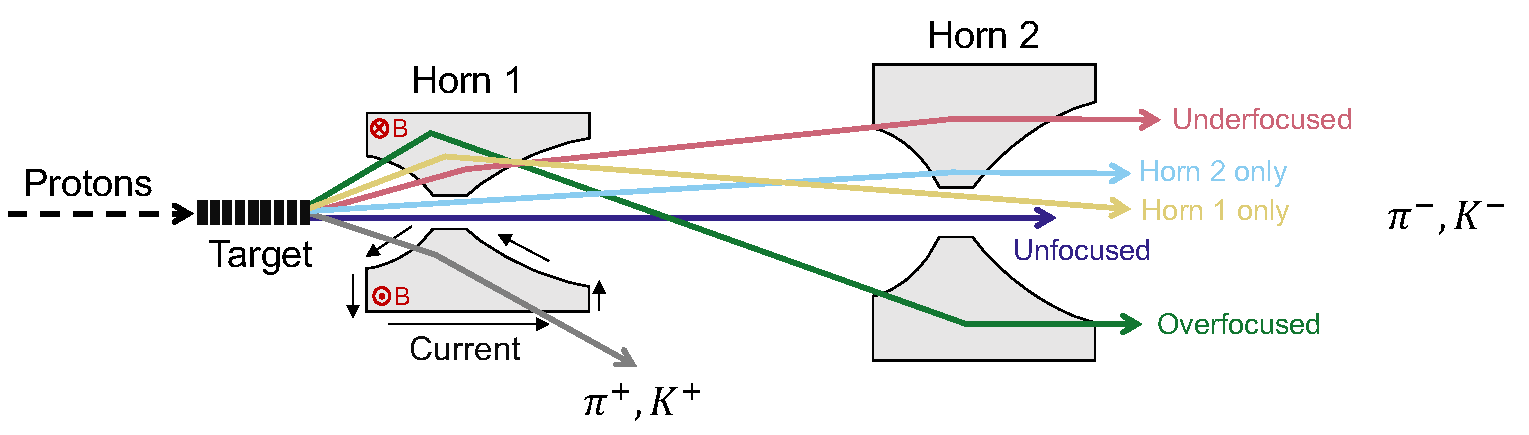
\includegraphics[width=1.\textwidth]{03minerva/figures/horns.pdf}}%
    \caption{Schematic of the working principle of the magnetic horns for the reverse horn current configuration indicating some possible trajectories, drawn based on the information provided in Ref.~\cite{AliagaSoplin:2016shs}. }
    \label{fig:horns}
\end{figure}

The first focusing horn perfectly focuses less than 10\% of charged hadrons producing antineutrinos, implying that the majority of hadrons require correction from the second focusing horn \cite{Bashyal:2021tzd}. Figure~\ref{fig:flux_focusComponents} illustrates the resulting antineutrino flux in both the ME configuration (used in this work's measurement) and the LE~configuration for comparison. Below 20~GeV, most antineutrinos are produced by pion decays, while antineutrinos produced from kaons dominate the high-energy tail. The bump observed at less than 1~GeV arises from low-energy antineutrinos produced by charged hadrons originating from outside the target. The rising part of the flux spectrum primarily originates from antineutrinos produced by charged pions that were initially overfocused by the first horn but subsequently corrected by the second horn. Conversely, the descending part of the flux corresponds to antineutrinos generated by underfocused charged pions, which are corrected by the second horn. 

\begin{figure}[t!] 
    \vspace{-5pt}
    \centering
    {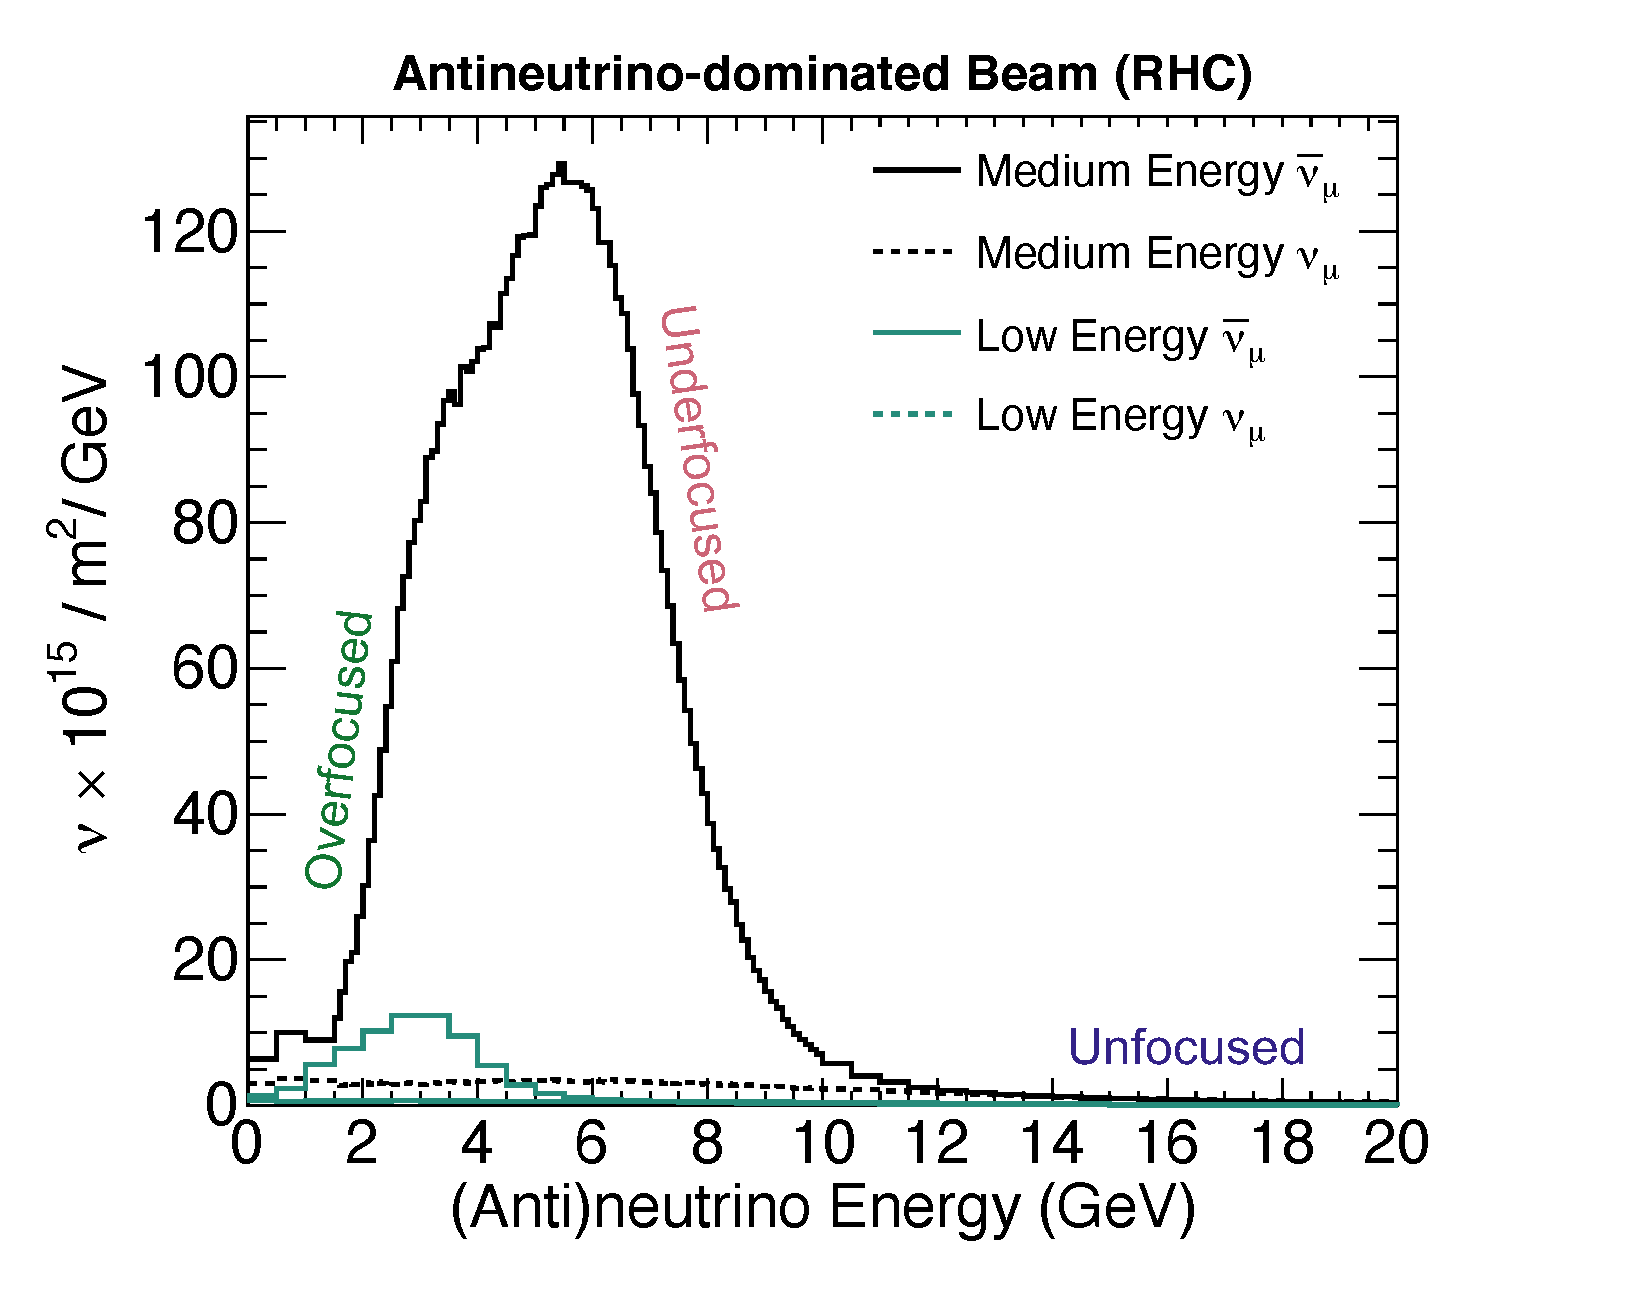
\includegraphics[width=.72\textwidth]{03minerva/figures/RHCflux_focusComponents.pdf}}%
    \caption{Distributions of (anti)neutrino fluxes in the medium and low energy regimes are depicted for the reverse horn current configuration at the MINERvA detector. These distributions represent the energy distributions of (anti)neutrino interactions per unit area. The solid lines represent the primary antineutrino contribution, while the dashed lines indicate neutrino contamination in the antineutrino-dominated beam. The contributions of specific antineutrino parent-focusing components are colour-coded to illustrate their trajectories in Figure~\ref{fig:horns}.}
    \label{fig:flux_focusComponents}
\end{figure}


Overall, the first horn predominantly focuses low-momentum charged pions, leading to the production of low-energy antineutrinos in comparison to the second horn. The inclusion of the second focusing horn significantly enhances the focusing, contributing to an increase of almost 50\% in the ME configuration \cite{Bashyal:2021tzd}. Some high-energy hadrons that are perfectly aligned with the magnetic horns can pass through without being charge-selected. Consequently, some of these hadrons decay into neutrinos, contributing to the contamination of the antineutrino-dominated beam, particularly at higher energies.

Focused negatively charged hadrons enter the 675~metres long decay pipe filled with helium to limit interactions with the hadron beam.~As they traverse the decay pipe, the hadrons primarily decay into muon antineutrinos via modes such as $\pi^{-}\rightarrow \mu^{-}\bar{\nu}_{\mu}$ with a~branching ratio exceeding 99\% and $K^{-}\rightarrow \mu^{-}\bar{\nu}_{\mu}$ with a branching ratio of 63.5\% \cite{numi2016_ADAMSON2016279,Workman:2022ynf}. The muon antineutrino beam is contaminated by $\nu_{\mu}$, $\nu_{e}$, and $\bar{\nu}_{e}$ due to other decay modes such as $K^{-}\rightarrow e^{-}\bar{\nu}_{e}\pi^{0}$ or $\pi^{-}\rightarrow \mu^{-}\bar{\nu}_{\mu} \rightarrow e^{-}\bar{\nu}_{e}\nu_{\mu}\bar{\nu}_{\mu}$ \cite{Workman:2022ynf}. Any remaining undecayed hadrons are detected by the hadron monitor and absorbed in the downstream\footnote{Downstream and upstream indicate positions relative to the beam direction, where downstream is in the direction of the beam, and upstream is against it.} hadron absorber made of aluminium, steel, and concrete. The only particles left in the beam---muons and antineutrinos---travel through 240~metres of dolomite rock interlaid  with four muon monitors as depicted in Figure~\ref{fig:numi}.\enlargethispage{2\baselineskip} 
The rock acts as a muon shield stopping the residual muons and allowing the antineutrinos to pass downstream to the MINOS near detector hall, which housed the MINERvA detector, located about 1~kilometre from the target. Some antineutrinos interact with the rock, creating additional antimuons referred to as rock muons, which could travel downstream to the MINERvA detector as well.
% rock muon - what they are
% Upgrade to fermilab beam line for NOvA ,where I got the number for the parameters
%https://ieeexplore.ieee.org/stamp/stamp.jsp?tp=&arnumber=4440873
% bunch is created around a particle which goes around the synchrotron with the frequency synced with the RF cavity
% beam description
% https://inspirehep.net/files/de0505656dd53c8c966da8531af0b55a
%hydrogen ions (H$^-$) are first accelerated to 400~MeV in the linear accelerator (Linac) and then converted into protons by passing through a carbon foil, which strips off the extra electrons going into the Booster, where they are subsequently further accelerated to 8~GeV. 

% https://lss.fnal.gov/archive/2015/pub/fermilab-pub-15-253-ad-fess-nd.pdf


\subsection{Simulation and characterisation}

% ME focusing uncertainties
% https://minerva-docdb.fnal.gov/cgi-bin/sso/ShowDocument?docid=16092
% ME hadron production uncertainties 
% page 228 - downloaded as eps and converted to pdf from 
% https://minerva-docdb.fnal.gov/cgi-bin/sso/ShowDocument?docid=12026

Precise knowledge of the (anti)neutrino flux produced by the NuMI beamline is crucial for (anti)neutrino cross-section measurements. In addition to determining the number of (anti)neutrinos that interacted in the detector, understanding how many were initially present in the beam is essential, as indicated in Equation~\ref{eq:xsec1D} in the following chapter. However, understanding the (anti)neutrino beam is challenging, primarily due to the complex processes involved in hadron production and the focusing components of the beamline. MINERvA addresses this challenge by employing a calculated \textit{a priori} flux, i.e. simulated flux adjusted using external hadron production data with varying parameters related to both hadron production and focusing to incorporate relevant systematic uncertainties. Direct flux measurements are also possible \cite{Loiacono2010} but are limited to an accuracy of 15\% due to poorly constrained backgrounds and detector uncertainties. 


The NuMI beam is simulated using the G4NuMI package, which is based on the GEANT4 (GEometry ANd Tracking) software version 9.4.p02~\cite{Geant4_AGOSTINELLI2003250,Geant4_1610988}, incorporating detailed geometrical models of the beamline.~The G4NuMI package, initially developed for MINOS \cite{Pavlovic2008, Koskinen2009, Loiacono2010}, was subsequently improved by MINERvA \cite{AliagaSoplin:2016shs, PhysRevD.94.092005}. It covers the entire process from the 120 GeV/$c$ protons impinging onto the graphite target to focused charged hadrons decaying into (anti)neutrinos, predicting the number, flavour, and momentum distributions. The underlying phenomenological hadronic models FRITIOF precompound \cite{Andersson:1986gw, Nilsson-Almqvist:1986ast} and Bertini cascade \cite{Bertini1963_PhysRev.131.1801,Guthrie:1968ue, Bertini1969_PhysRev.188.1711,BERTINI1971670} implemented in the FTFP\_BERT package of GEANT4 to predict the hadrons produced by the proton-carbon interactions were, however, shown to disagree with external hadron production data \cite{AliagaSoplin:2016shs}.
Therefore, MINERvA developed the Package to Predict the Flux (PPFX) \cite{AliagaSoplin:2016shs,Aliaga_2014} to constrain these models using external experimental data. 


%The PPFX primarily uses the NA49 \cite{Alt_2007} and the MIPP \cite{PhysRevD.90.032001} pion production datasets, which are corrected to the NuMI appropriate energy scale using the FLUKA simulation \cite{Ferrari:2005zk, BOHLEN2014211}. The NA49 experiment at CERN measured the pion production on a thin, i.e.~a~few percent of interaction length, carbon target using a 158~GeV/$c$ proton beam \cite{Alt_2007}. The MIPP experiment measured pion production on a replica of the LE NuMI target (about 2~proton interaction lengths) using a 120 GeV/$c$ protons \cite{PhysRevD.90.032001}. Additional datasets are also employed in the PPFX to constrain kaon and nucleon production, as well as the absorption of particles in beamline materials as described in detail in Ref.~\cite{PhysRevD.94.092005}.

% MIPP not used because thick target constraint doesn't agree with low nu method

The PPFX primarily uses the NA49 \cite{Alt_2007} pion production dataset, which is corrected to the NuMI appropriate energy scale using the FLUKA simulation \cite{Ferrari:2005zk, BOHLEN2014211}. The NA49 experiment at CERN measured the pion production on a thin, i.e.~a~few percent of interaction length, carbon target using a 158~GeV/$c$ proton beam \cite{Alt_2007}. \enlargethispage{1\baselineskip}Additional datasets are also employed in the PPFX to constrain kaon and nucleon production, as well as the absorption of particles in beamline materials as described in detail in Ref.~\cite{PhysRevD.94.092005}. Uncertainties from each of these datasets are incorporated in the hadron production correction reweight of the base simulation. For interactions with no available data, the uncertainty is evaluated using the spread of various hadronic models in GEANT4. 

\begin{figure}[t!] 
    \vspace{-20pt}
    \centering
    {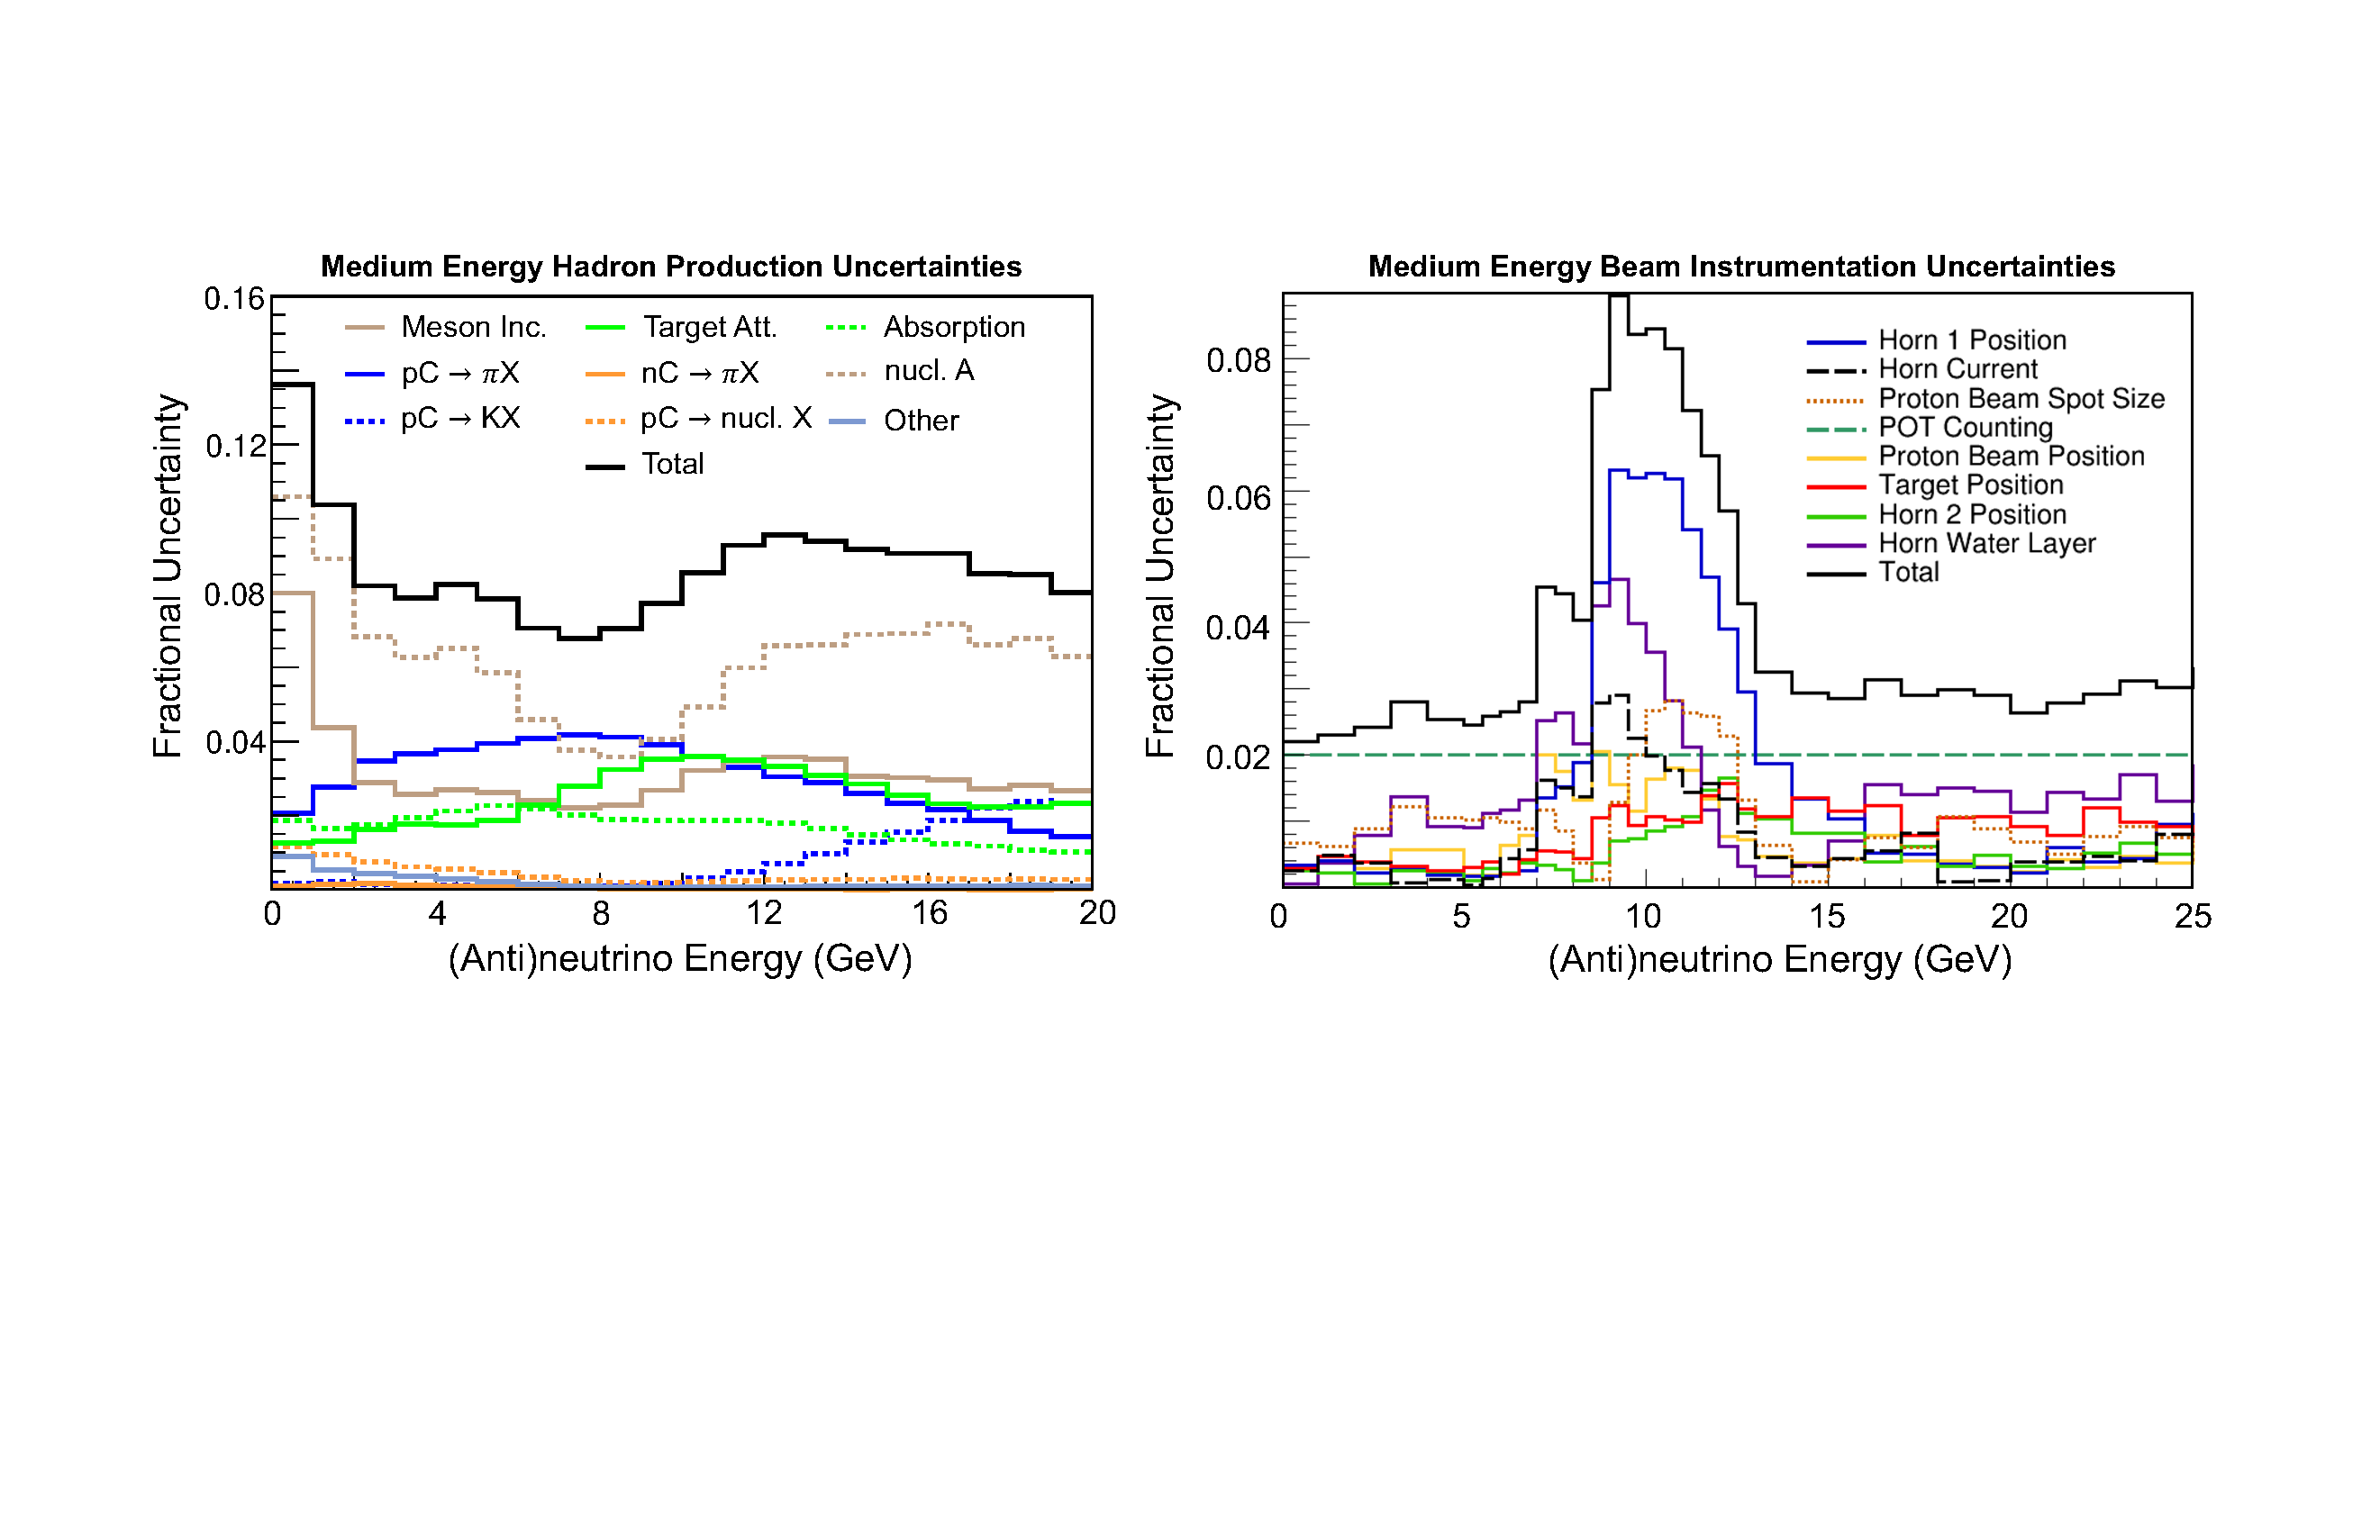
\includegraphics[width=1\textwidth]{03minerva/figures/ppfx_unc.pdf}}%
    \caption{PPFX uncertainties on the NuMI medium energy flux. Left: Flux uncertainty from different hadron interaction categories modified from Ref.~\cite{AliagaSoplin:2016shs}. Note that `Meson Inc.' refers to the uncertainty of mesons interacting on any material in the beamline, `Target Att.' and `Absorption' are the uncertainties due to the absorption of particles in the target and other materials, respectively, `nucl. A' represents mainly nucleons interacting in material that is not carbon, and `Other' includes any other interactions. Right: Beam geometry and focusing uncertainties modified from Ref~\cite{Messerly:2019itw}. `Baffle Scraping' represents the uncertainty on the tails of the proton beam interacting with the baffle.}
    \label{fig:ppfx_unc}
\end{figure}

The hadron production uncertainties are then propagated to the (anti)neutrino energy distribution using a so-called multiverse method \cite{MAT_Messerly_2021}.~A collection of 100 flux predictions, referred to as universes, is created by randomly sampling from a multidimensional Gaussian distribution centred on the default parameter values of hadron production cross-sections varied within their uncertainties and taking into account correlations between the parameters. The spread of the universes in each bin provides the \textit{a priori} flux uncertainties arising from the hadron production, as depicted in Figure~\ref{fig:ppfx_unc} for the NuMI beam in medium energy.

Furthermore, PPFX also enables the implementation of uncertainties arising from beamline instrumentation, such as the position of the target relative to the horn, the current applied to the magnetic horns, or the residual water layer on horns due to cooling. \enlargethispage{1\baselineskip}These uncertainties can be evaluated similarly to the hadron production uncertainties and are also depicted in Figure~\ref{fig:ppfx_unc} for the NuMI beam in medium energy. Overall, the flux uncertainty is dominated by hadron production, except in the falling edge of the (anti)neutrino distribution, where focusing uncertainties dominate. Additionally, MINERvA also improves the flux through \textit{in-situ} measurements of processes with known cross-sections, as discussed in Chapter~\ref{ch:dataAsimulation}.


\section{MINERvA detector}\label{sec:MINERvAdetector} 

\begin{figure}[b!] 
    \centering
    {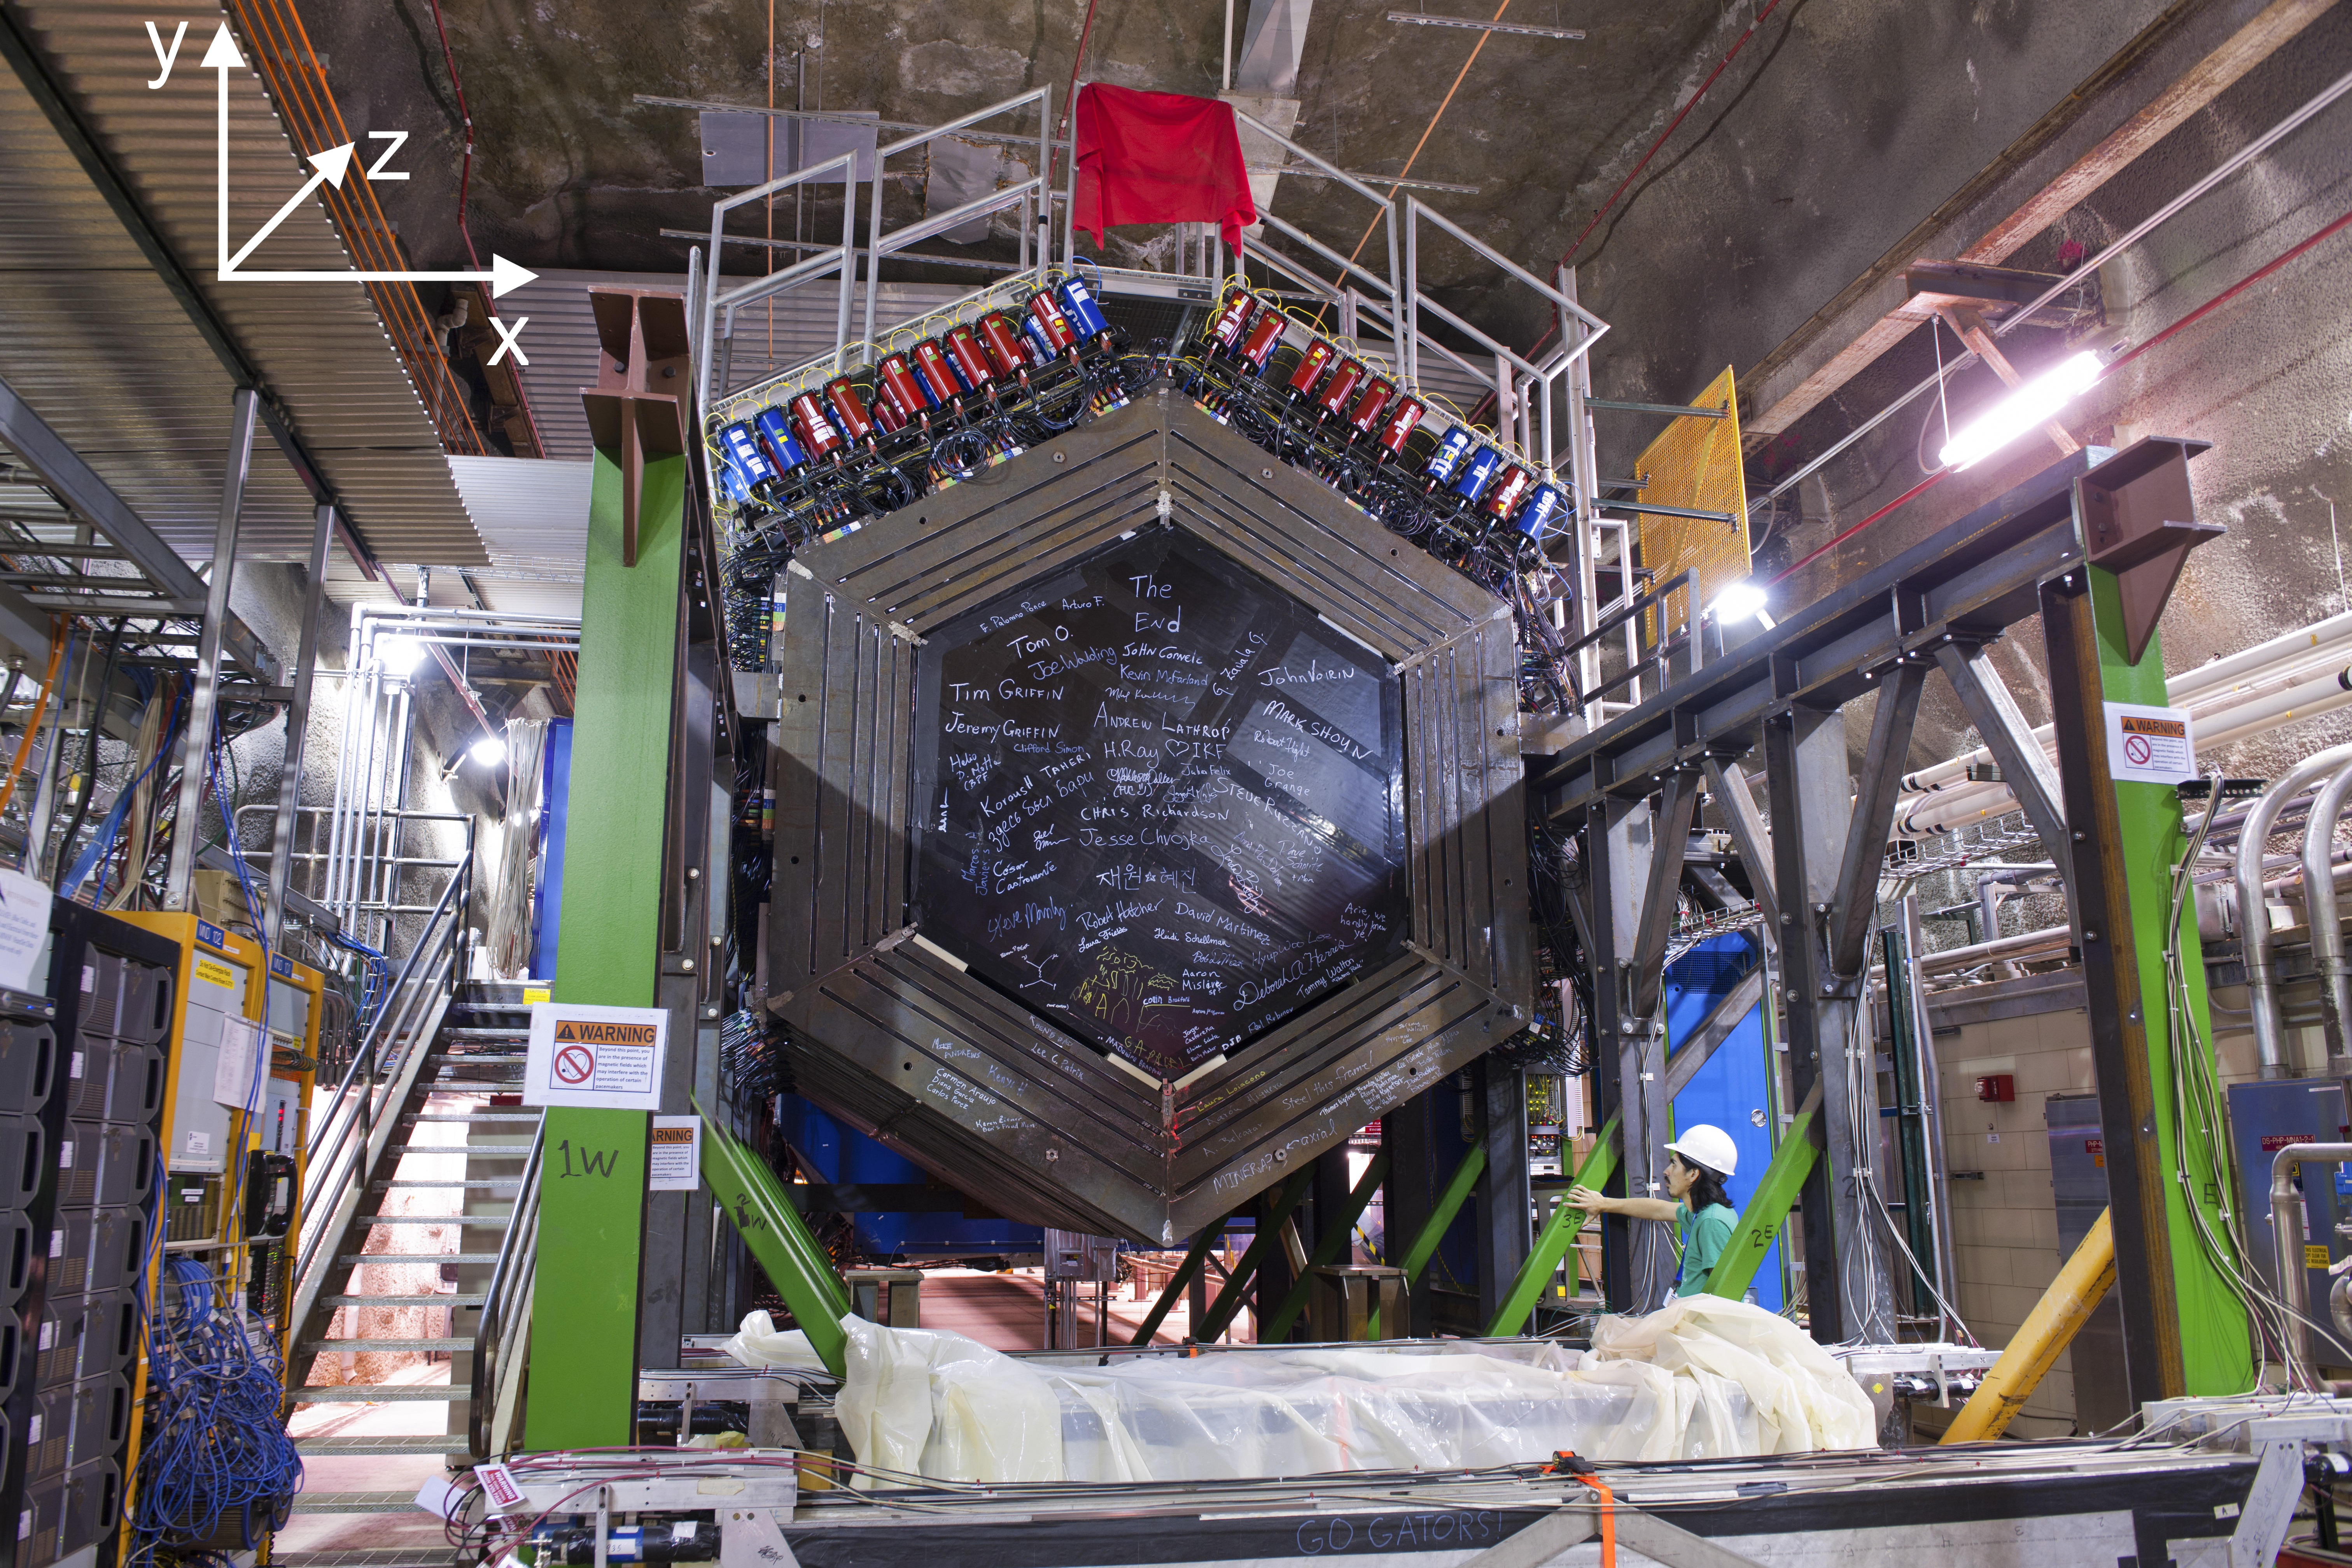
\includegraphics[width=0.9\textwidth]{03minerva/figures/minerva_photo.jpg}}%
    \caption{Photo of the front view of the MINERvA detector showing the last installed module. The signed black plane is the inner detector, while the metal frame around is the outer detector. The red and blue cylinders on the top of the detector depict the optical readout system. Permission to reuse granted by Fermilab Creative Services. Credit: Reidar Hahn, Fermilab.}
    \label{fig:detectorPhoto}
\end{figure}


The MINERvA detector~\cite{Aliaga_2014} was located approximately 100~metres underground in the MINOS near detector hall and about 1~kilometre away from the graphite target of the NuMI beamline. As shown in Figure~\ref{fig:detectorPhoto}, MINERvA itself was a hexagonal detector made of an inner detector part in black that is mounted within a metal outer detector frame. On the top of the frame, there was an optical readout system in red and blue. \enlargethispage{1.5\baselineskip}The detector design and methods of operations were fundamental in enabling MINERvA to identify and study (anti)neutrino interactions.

Akin to other particle detectors, MINERvA worked like a very fast camera, capturing `snapshots' in both space and time of the energy deposited in the detector by particles resulting from interactions between (anti)neutrinos and the detector material. An example of such a `snapshot', referred to as an event, is shown in Figure~\ref{fig:eventDisplayDIS}. MINERvA's detection capability depended on two key elements: first, the use of finely segmented solid plastic scintillator technology for the active regions, enabling the measurement of energy deposits; and second, fast timing resolution ($\sim$5 ns) to distinguish overlapping events within a single spill, determining how quickly and frequently MINERvA could capture these `snapshots'.


\begin{figure}[t!] 
    \vspace{-15pt}
    \centering
    {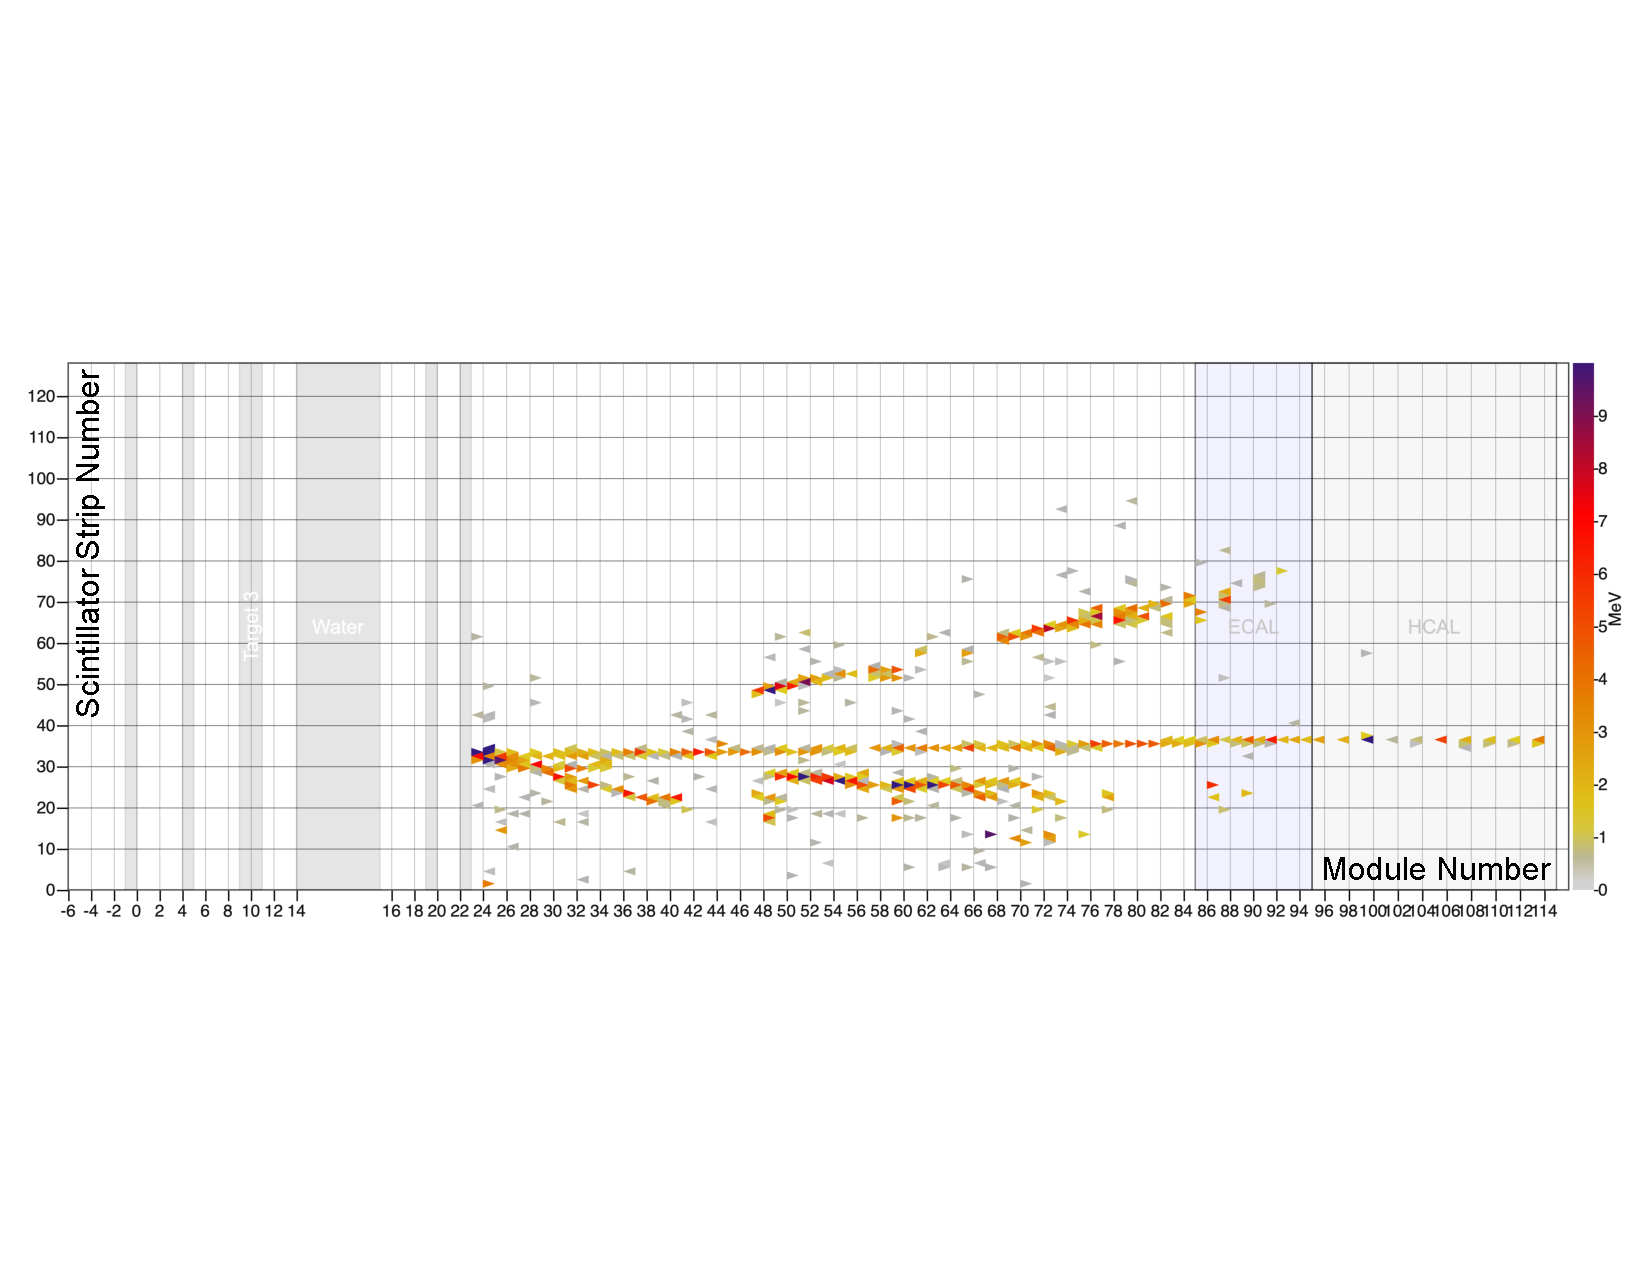
\includegraphics[width=1\textwidth]{03minerva/figures/dis_eventDisplay_new.pdf}}%
    \caption{Simulated antineutrino deep inelastic scattering (DIS) interaction in the MINERvA detector. The antineutrino interacts with a lead nucleus in target 5, producing an antimuon (the longest track) and multiple hadrons showers. The individual triangles are the energy deposits with their colour representing the size of the deposit.~The $x$-axis depicts the detector module number along the general direction of the beam. }
    \label{fig:eventDisplayDIS}
    \vspace{-2pt}
    %$\mu^{+}$ 3 protons, 2 $\pi^{0}$ and neutron
\end{figure}

MINERvA used a right-handed coordinate system with an origin at the centre of the detector, which is superimposed on the front view of the detector in Figure~\ref{fig:detectorPhoto}. In this system, the $z$-axis pointed downstream along the central axis of the detector, $y$-axis was pointed upwards, and the $x$-axis was directed to the left from the perspective of the beam. The (anti)neutrino beam itself, therefore, pointed 3.34$^{\circ}$ downwards in the $y$-$z$~plane. 

Figure~\ref{fig:detectorView} shows a schematic of the complete side view of the detector. As depicted, the upstream part of the inner detector consisted of the nuclear target region including carbon, iron, lead and water interleaved between the plastic scintillator planes, enabling the study of nuclear effects in (anti)neutrino interactions.\enlargethispage{2\baselineskip}~The main fiducial volume comprised the central tracking region, composed purely of finely segmented plastic scintillator planes to resolve and identify multi-particle final states, as well as track low-energy particles with energies greater than about 100~MeV. 

\begin{figure}[t!] 
    \vspace{-8pt}
    \centering
    {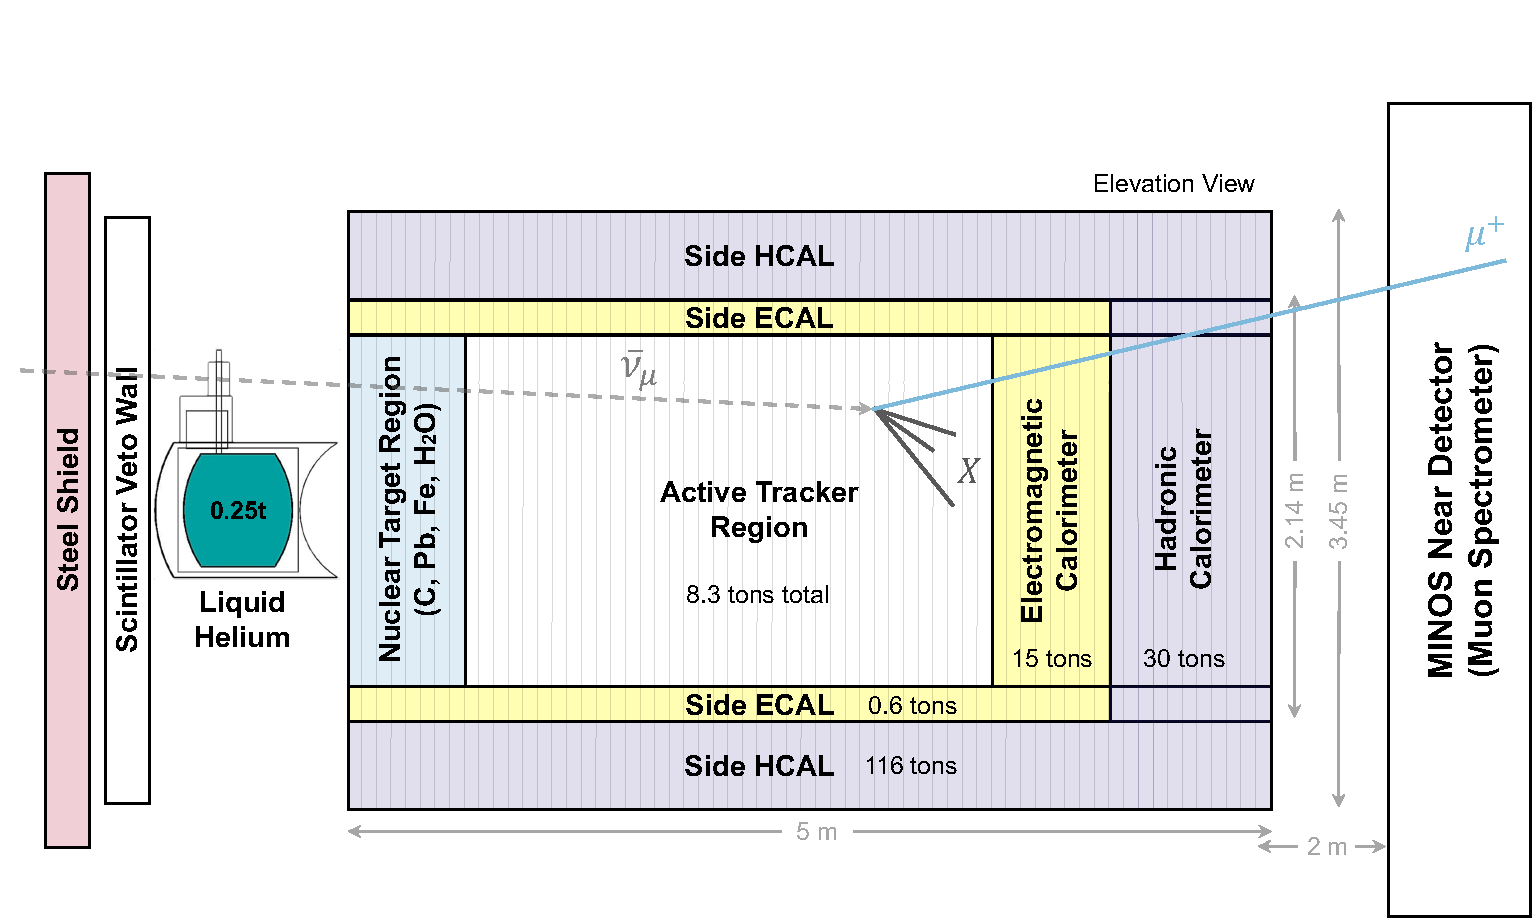
\includegraphics[width=1\textwidth]{03minerva/figures/minerva_view.pdf}}%
    \caption{Schematic side view of the MINERvA detector. Modified from Ref.~\cite{Aliaga_2014}.}
    \label{fig:detectorView}
\end{figure}

To contain electromagnetic showers and high-energy hadronic final states in the direction of the beam, the tracker was followed by alternating layers of lead--scintillator and steel--scintillator in the sampling electromagnetic (ECAL) and hadronic calorimeter (HCAL), respectively. Additionally, the outermost 15~cm of each ID plane was covered by steel side ECAL to reduce the amount of energy leaving the ID in the $x$-$y$~plane. For full containment and also acting as a support structure, the ID was surrounded by the outer detector (OD) lead hadronic calorimeter with four embedded scintillator strips visible in Figure~\ref{fig:detectorPhoto}.

MINERvA was able to tag the highly-energetic rock muons before they entered the detector and reject low-energy hadrons produced in the rock using a veto wall upstream of the main detector, consisting of a steel shield and scintillator. Between the veto wall and the front face of the main body of the detector, there was a liquid helium target in an aluminium cryostat, offering opportunities to measure (anti)neutrino interactions with somewhat less complicated and more easily predicted nuclear effects than heavier targets. The MINOS near detector, located downstream of the main MINERvA detector, functioned as a spectrometer for (anti)muons that were not contained within the MINERvA detector. This is further discussed in Section~\ref{sec:MINOS}.

% add plane numbers
% 20 ECAL
% 10 HCAL

\subsection{Scintillator planes}

Each hexagonal plane of the ID was made of 127 triangular solid scintillator strips of variable lengths of $\mathcal{O}$(1~m) stacked in the $x$-$y$~coordinate plane. Depending on the arrangement of the strips, there were three possible plane orientations, $X$, $U$, and $V$, referred to as views, which are illustrated in Figure~\ref{fig:scintillator}. The $X$-view consisted of scintillator strips running in parallel to the $y$-axis, whereas $U$- and $V$-view had strip arrangement rotated 60$^{\circ}$ clockwise and anticlockwise from the $X$-view, respectively. Figure~\ref{fig:scintillator} also shows the stacking of different views in the detector, where each $X$-view is alternately followed by either a $U$- or $V$-view. A so-called tracking module is formed by two planes, either $XU$ or $XV$. Although typically only two orthogonal planes (along with the time dimension) are required for three-dimensional reconstruction, the three different views provided an opportunity to mitigate potential ambiguities in reconstructed hit associations seen when multiple tracks traverse two orthogonal planes. 


\begin{figure}[b!] 
    \vspace{-5pt}
    \centering
    {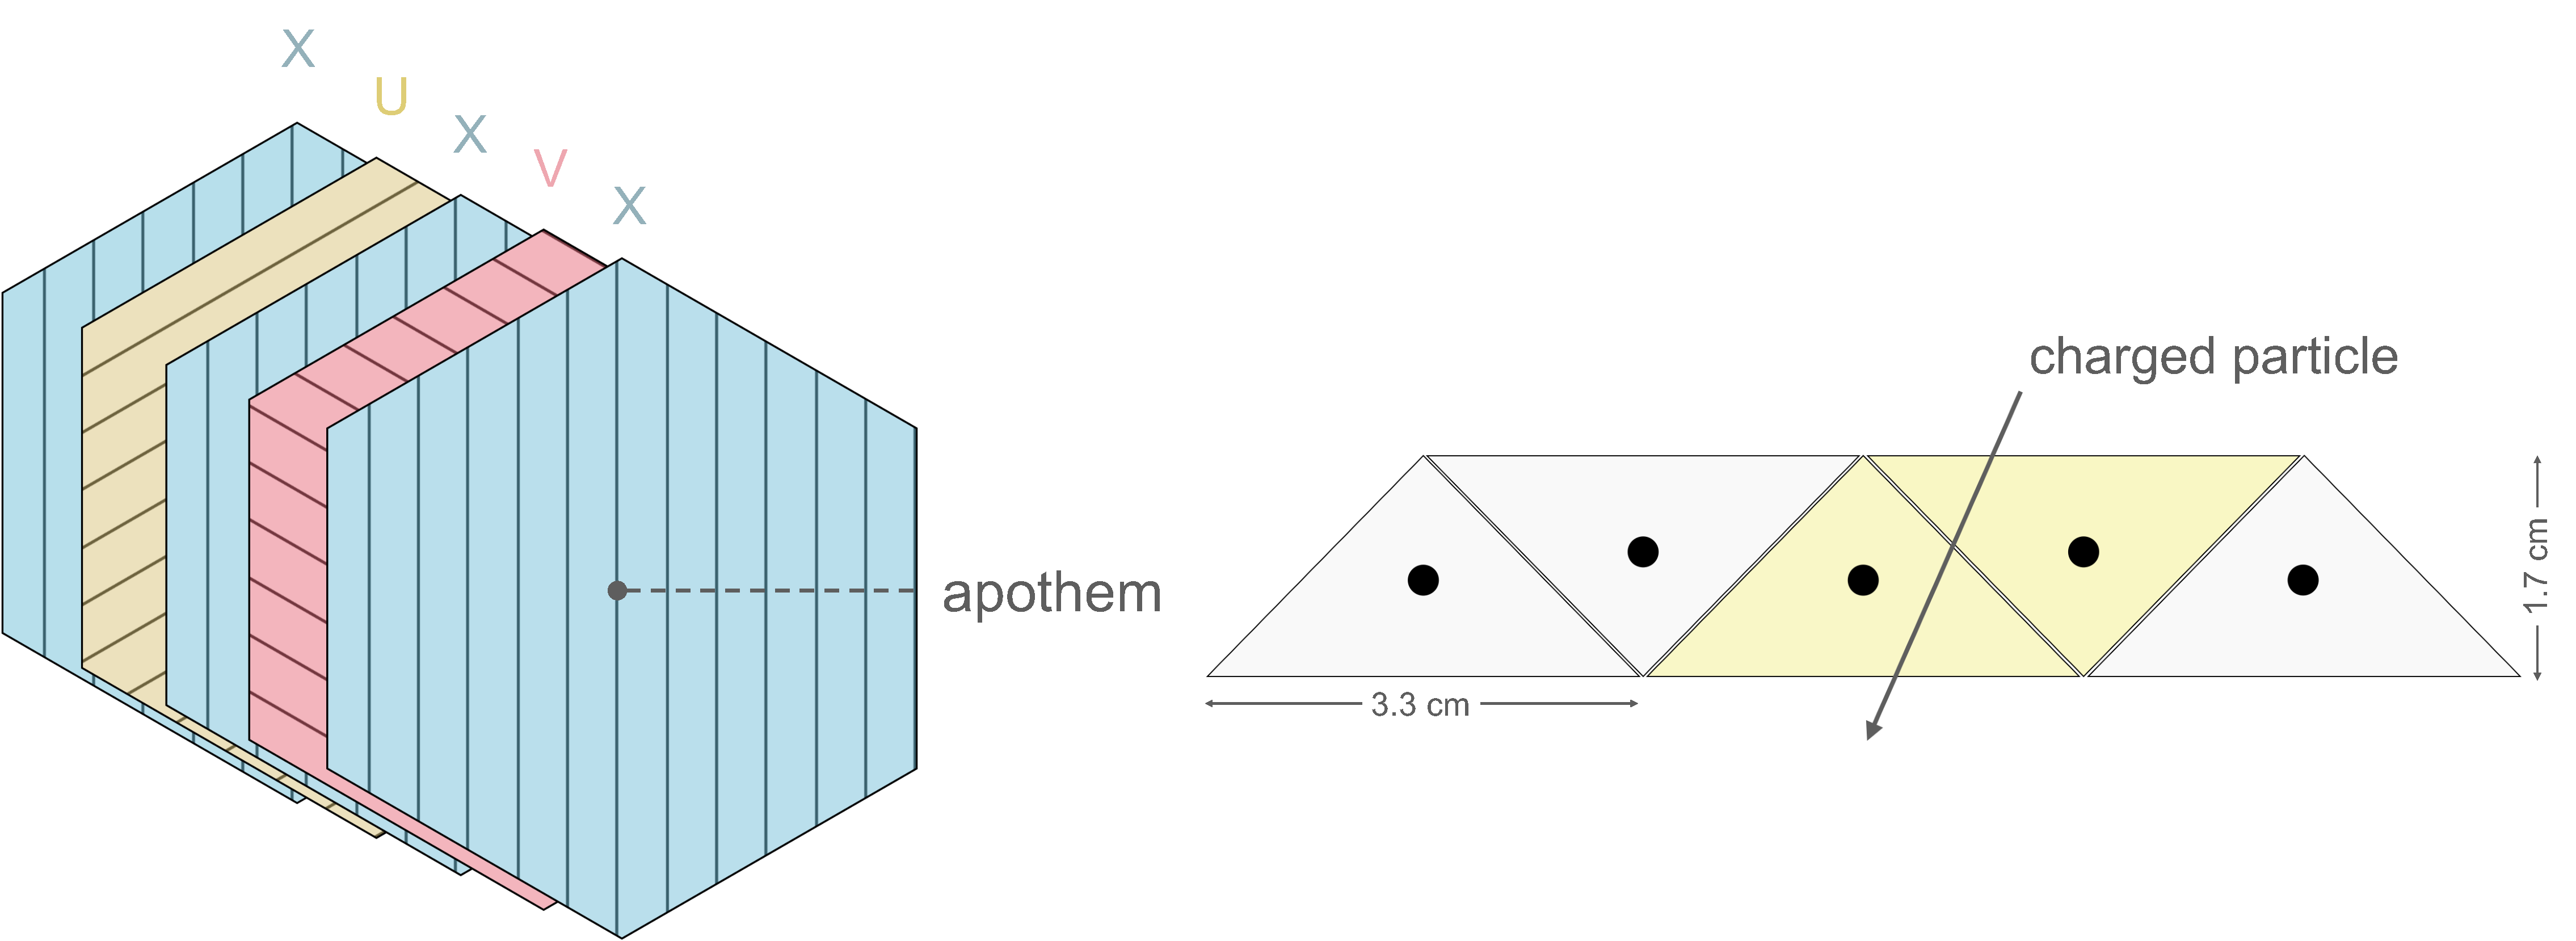
\includegraphics[width=1\textwidth]{03minerva/figures/scintillator.pdf}}%
    \caption{Left: Diagram of the three views of scintillator planes and their stacking in the detector. Right: Cross-section of the configuration of triangular scintillator strips, i.e. bars, making up one scintillator plane, showing the impact of a charged particle passing through.}
    \label{fig:scintillator}
\end{figure}


The individual scintillator strips, primarily made of doped polystyrene, i.e. hydrocarbon (CH), were glued and sealed together light-tight with epoxy to prevent light leaks. Additionally, polycarbonate sheets were applied to enhance the overall rigidity of the assembly. Each scintillator strip was also coated by reflective titanium dioxide for optical isolation. \enlargethispage{1\baselineskip}Figure~\ref{fig:scintillator} demonstrates that the triangular strips were overlaid in such a way that a charged particle passing through a plane would deposit energy and hence create a scintillation signal, i.e.~blue light, in at least two scintillator strips. The scintillation light was collected via wavelength shifting (WLS) fibres at the centre of each strip further discussed in Section~\ref{sec:opticalReadout}. 

Note that in contrast to the ID, the scintillator strips embedded in the OD were rectangular with bigger cross-sections.

\subsection{Nuclear target region}

MINERvA's unique capability to perform self-contained measurements of nuclear dependence in (anti)neutrino scattering stems from the nuclear target region. It was composed of five solid passive, i.e. not instrumented, targets made of transverse segments of carbon~(C), iron~(Fe), and lead~(Pb), interlaid with tracking modules (made of two scintillator planes each) as depicted in Figure~\ref{fig:targetRegion}. While the geometry of the individual targets may seem complex, it, for example, allowed for the investigation of acceptance differences at various regions of the detector due to the MINOS near detector acceptance constraint discussed later on in Section~\ref{sec:MINOS}. Furthermore, the patterns were chosen so that (anti)neutrinos that did not interact within the nuclear target region would traverse approximately the same amount of material throughout the target region, irrespective of their trajectory in the $y$-$z$~plane. 

\begin{figure}[t!] 
    \vspace{-5pt}
    \centering
    {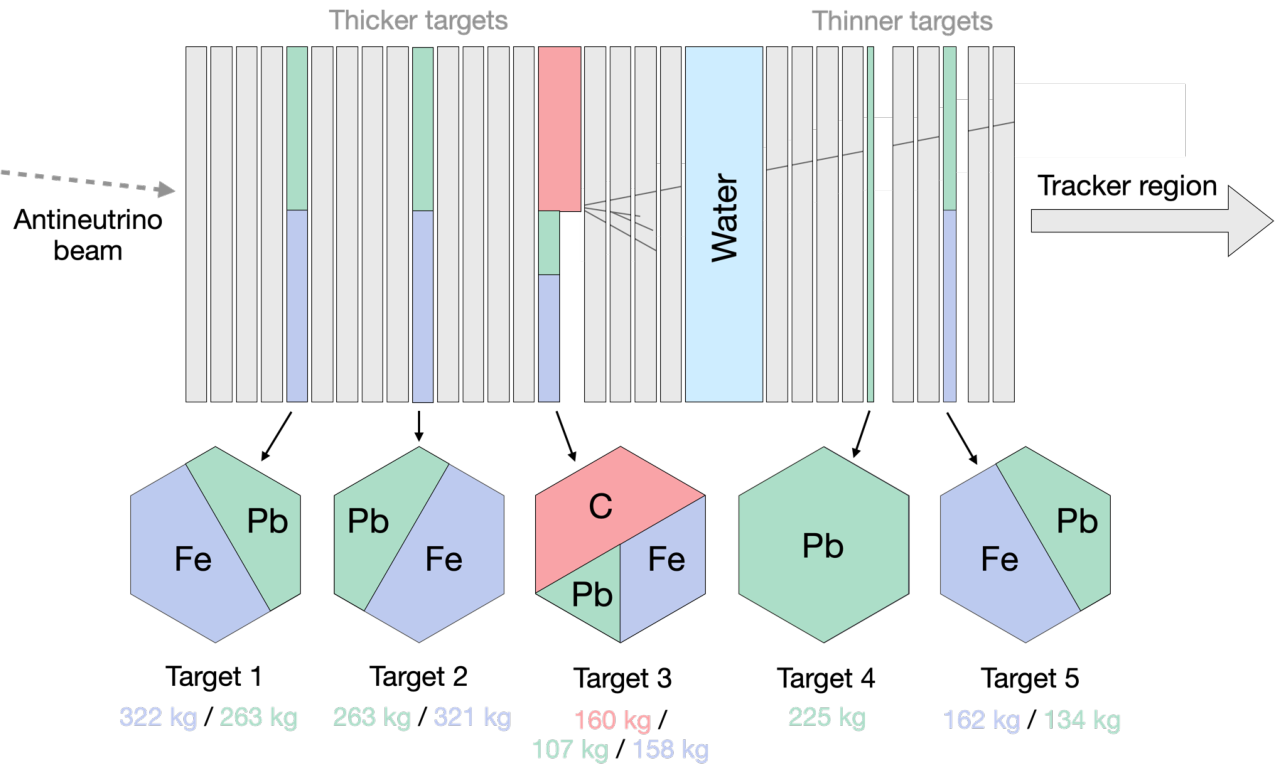
\includegraphics[width=1\textwidth]{03minerva/figures/targetRegion.pdf}}%
    \vspace{10pt}
    \caption{Diagram of the nuclear target region in the MINERvA detector. The individual target cross-sections are depicted looking downstream of the detector. The fiducial mass information was taken from Ref.~\cite{Aliaga_2014}.}
    \label{fig:targetRegion}
\end{figure}

Figure~\ref{fig:targetRegion} also shows the geometrical division of the individual target planes into different materials as visible when looking downstream of the detector. Both targets 1 and~2 were composed of roughly 60\% iron and 40\% lead in terms of fiducial area, with a plane thickness of about 2.6~cm (about one tracking module). However, they contained nearly the same amount of fiducial mass of iron and lead. The orientation of iron and lead in target 2 was flipped horizontally, i.e.~reflected around the $y$-axis, with respect to target 1. As the most upstream target, target 1 was affected by a limited number of upstream tracking planes used to identify particles produced outside the MINERvA detector, particularly the rock muons. This aspect is relevant in the context of this work's measurement discussed later in Section~\ref{sec:eventSelection}.

Target 3 consisted of 50\% carbon, approximately 33\% iron and 17\% lead, i.e. 1/3 iron and 1/6 lead, respectively, allowing for detailed studies of nuclear dependence in (anti)neutrino scattering within one target. The carbon provided valuable cross-validation for the (anti)neutrino interaction cross-sections in plastic scintillator (hydrocarbon) and vice versa, as they are expected to be approximately the same. In general, (hydro)carbon data was crucial for comparison with results from other experiments such as T2K~\cite{t2k_ABE2011106}. Target 3 was the thickest of all the solid targets to ensure sufficient fiducial mass for the light carbon. The iron and lead parts had the same thickness as in targets 1 and 2, while the carbon component was about 7.6~cm thick. All materials were aligned at the upstream end, resulting in an air gap downstream of the iron and lead components. 

Target 4, the thinnest in the series (comprising less than 1/3 of a tracker module), was constructed using pure lead to ensure the conversion of any produced photons from either upstream or downstream targets. The chosen thickness, approximately 1.5 radiation lengths, allowed photons to initiate a shower but not enough to be fully contained. This strategy improved event containment in the upstream targets and concurrently reduced noise from photons (or $\pi^0$s and neutrons), minimising potential confusion in tracker reconstruction and event selection. Its reduced thickness resulted in an air gap between the target and the first downstream scintillator plane. 

Target 5, located directly upstream of the fully active tracking region, had the same shape as target 1 but only half of its thickness (about half of a tracker module). It was designed for the study of lower-energy particles and particle multiplicities, benefiting from enhanced tracking and energy resolution. Similar to targets 3 and 4, there was an air gap between target 5 and the following tracker module, which also allowed for better spatial separation of low-energy final state particles. 

Placing thicker targets upstream was done to minimise interference with particles resulting from interactions in downstream targets, thereby optimising the reconstruction of (anti)neutrino interactions and their exclusive final states.

In addition, there was a water target located between the solid targets 3 and 4. It consisted of a circular neoprene balloon filled with (liquid) water suspended on a circular steel frame and held in place with sheets made of polyamide synthetic fibre. The water target thickness varied between 17~cm at the edge of the balloon to 24~cm at the centre of the balloon, with the water volume measured when the target was emptied. The water target is not included in this work's measurement, similar to the helium target described earlier.

In general, each target was separated by four tracking modules, except target 4 and target 5, which were separated by only two tracking modules. \enlargethispage{1\baselineskip} Figure~\ref{fig:targetRegion} demonstrates how the active layers between the targets enabled the identification of the location of (anti)neutrino interactions and tracking of final state particles. 

\subsection{Optical readout and data acquisition}\label{sec:opticalReadout}

A wavelength-shifting (WLS) fibre embedded in the centre of each scintillator strip absorbed the produced blue scintillation light, re-emitting it inside the fibre as green. The WLS fibres then directed the light out of the detector, connecting to clear optical fibres. The shifted green light was reflected internally within the fibre as it travelled, minimising the signal reduction, while the end of the fibre not pointed towards the readout system was mirrored to reflect the light back.

The clear optical fibres from adjacent scintillator strips were grouped in sets of eight. Eight sets of these optical fibre groups were connected to one photomultiplier tube (PMT) with 64 channels, i.e., an 8×8 array of pixels, which converted the collected light into charge. The fibres were interleaved in such a way that the light signal from adjacent scintillator strips did not go into adjacent pixels of the PMT to prevent signal cross-talk. The PMT converted collected photons into photoelectrons via the photoelectric effect on its photocathode, wherein light incident on a metal surface with energy above the material's binding energy ejected electrons. Subsequently, the electrons were multiplied going through a chain of dynodes with high potential differences between succeeding dynodes. Electrons collided with each anode, producing more electrons, which eventually reached the anode end of the tube, resulting in a sharp current pulse that was easily measurable. 

MINERvA had about $\sim$500~PMTs totalling approximately~32~000 channels. Each PMT was enclosed in a light-tight cylindrical steel enclosure visible on top of the detector in Figure~\ref{fig:detectorPhoto}. Each PMT was read out by one front-end board (FEB), which performed the timing and pulse-height signal digitisation, so-called time-to-digital (TDC) and analog-to-digital (ADC) conversion. MINERvA's readout was synchronised with the NuMI beam spill timing. The readout window, referred to as the gate, was 16~$\mu$s long, starting 0.5~$\mu$s before the beam spill and adding an extra 5.5~$\mu$s after the beam arrived to include delayed activity from (anti)neutrino-produced meson decays. MINERvA also triggered on beam-off data every $\sim$1500~beam spills to measure the beam-off background and calibrate the detector. Note that channels had a 20~ns long reset time after being fired, rendering them essentially dead to any incoming signals. A full description of the MINERvA data acquisition (DAQ) system can be found in Ref.~\cite{DAQ_PERDUE2012179}.

\section{Calibration}\label{sec:calibration}

A detector calibration allowed retrieving information from the ADC and TDC counts obtained from the DAQ system needed for further physical interpretation. For example, the ADC counts represented energy deposits but were essentially only digits without proper conversion to energy.~Calibration also addressed various effects that could introduce biases to these conversions.~MINERvA, therefore, calibrated the various detector components both \textit{ex-situ} prior to installation in the detector and \textit{in-situ} during its run, as described in detail in Ref.~\cite{Aliaga_2014}.%Similarly, TDC counts require adjustment for relative timing offsets among various detector parts.

In order to be able to convert ADC counts back to charge in reconstruction, all FEBs were bench-tested outside the detector using the same (known) charge injection, producing a response correction factor for each of the FEBs. Furthermore, the attenuation differences of the WLS fibres in different parts of the scintillator strip were measured \textit{ex-situ} using radioactive sources, resulting in attenuation corrections as a function of the position of the energy deposit. 
% to map the ADC-to-charge conversion response curve used in reconstruction.

\textit{In-situ} calibrations were necessary to characterise time-dependent effects. The pedestal ADC count, originating from the inherent background noise levels of the readout electronics and PMTs, as well as background detector activity (such as cosmic rays and radioactivity), was measured during beam-off triggers roughly twice a day. In addition, the photoelectron multiplication strength, known as gain, of the PMTs was measured using a light injection system with a constant light source between each NuMI spill. This calibration process aimed to account for gain variation due to PMT ageing. 

%that generated roughly one photoelectron in each channel. 

During the detector run, numerous MINERvA calibrations also made use of rock muons. Muons, being minimum ionising particles, generally exhibit a consistent and well-understood energy deposition pattern in a detector. For example, rock muon tracks were used to identify dead strips in the detector, or to correct for variations in light yields between different scintillator strips, ensuring a uniform energy response throughout the detector. Rock muons were also instrumental in correcting the absolute energy scale of the detector by comparing muon peak energy deposits in both data and simulation. This correction factor, derived from the data-to-simulation ratio, evolved over time to compensate for scintillator and WLS fibre ageing. 

% timing
Finally, timing information was calibrated to account for the finite time it took for light to travel from the detector to the PMT, considering the length of the optical fibre. Additionally, a rock muon sample enabled the correction of time slewing caused by scintillator decay times, which are dependent on energy deposits, and any remaining channel-to-channel offsets between FEBs.

%The time of each hit is compared with the truncated mean time of hits on the track to form a residual, taking into account the travel time of the muon and previous timing calibrations. The calibration moves the center the peak of the hit time residual to 0. A separate time calibration accounts for the time offset between FEBs.


% NOT TALK ABOUT: 
% cross-talk: identified as signal measured in channels that were not traversed by the muon but sit on the same PMT as channels that were traversed by the muon.
% plane alignment
% target position

%Finally, the nuclear target position in the simulation described in Chapter~\ref{ch:dataAsimulation} based on a measurement survey at the edge of the detector was adjusted using events with two or more reconstructed tracks in data and simulation. This was done using the point of closet approach to be reconstructed within a nuclear target.  

\section{MINOS near detector}\label{sec:MINOS}

\begin{figure}[b!] 
    \centering
    {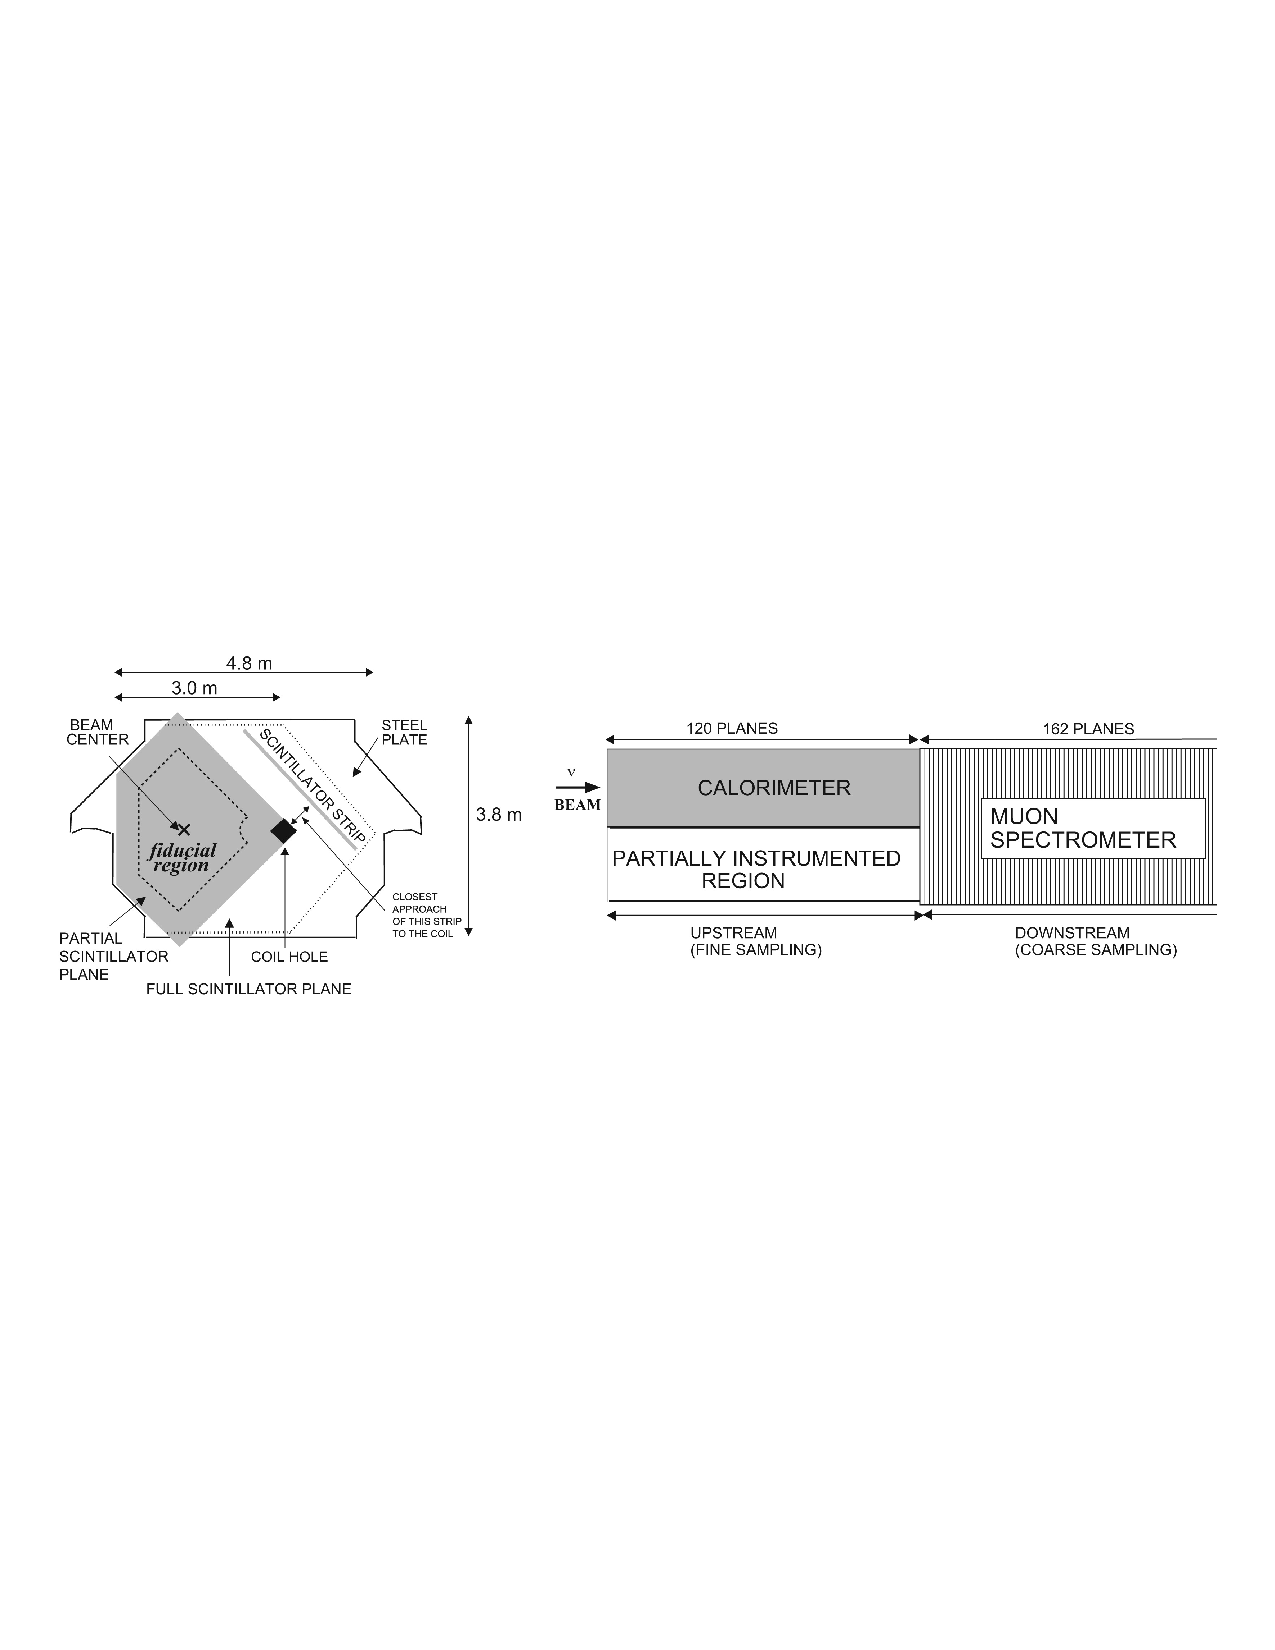
\includegraphics[width=1.\textwidth]{03minerva/figures/minos.pdf}}%
    \caption{Schematic view of the MINOS near detector. Left: Transverse view of the plane configuration looking downstream. The shaded area shows a partially instrumented active scintillator plane while the dotted line shows the outline of a fully instrumented scintillator plane. The black square represents the coil hole. Right: Top view of the MINOS near detector showing the partially instrumented calorimeter region and the muon spectrometer. Note that the partially instrumented region has a full coverage every fifth plane (like the muon spectrometer). Reprinted with permission from the MINOS collaboration \cite{PhysRevD.81.072002}. Copyright (2024) by the American Physical Society.}
    \label{fig:minos}
\end{figure}


While the design of the MINERvA detector allowed for tracking low-energy charged particles, the majority of GeV-scaled (anti)muons produced in charged-current interactions were not contained within the detector. Therefore, the physics program of the MINERvA experiment relied on the MINOS near detector shown in Figure~\ref{fig:minos} \cite{minos_MICHAEL2008190}, which was positioned 2~metres downstream of the MINERvA detector's hadron calorimeter. Crucially, although somewhat similar in design to the MINERvA HCAL, the MINOS near detector was magnetised, i.e. acting as (anti)muon spectrometer. This setup enabled precise momentum reconstruction of (anti)muons exiting the MINERvA detector volume in the forward direction.

The MINOS near detector \cite{minos_MICHAEL2008190} was a sampling calorimeter consisting of alternating planes of magnetised steel and segmented plastic scintillator, oriented in two different views to enable 3D reconstruction. The toroidal magnetic field of approximately 1.3~T was generated by a current-carrying coil spanning the entire length of the detector, as depicted in Figure~\ref{fig:minos}. Surrounding the coil, there was also a small region without the scintillator rendering this region effectively dead, which is not shown in the schematic. This aspect motivates part of the selection in this measurement, as discussed later on in Chapter~\ref{ch:analysis1D}. The optical readout system used the same PMTs as MINERvA. 

As a~charged \mbox{particle--—whether} it be an antimuon or a muon, aligning with MINERvA's scope of interest--—travelled through MINOS, it was deflected by the magnetic field. The momentum of the (anti)muon was then determined using the range and curvature of the track, while the direction of the curvature was used to specify its charge, i.e. whether it was a muon or an antimuon \cite{ospanov2008measurement}. In the context of this work, the latter is important for background removal from neutrinos produced in the antineutrino-dominated beam mode. A more detailed discussion about the reconstruction by range and curvature is included in Chapter~\ref{ch:Reconstruction}.

Considering the position and transverse dimensions of the MINOS detector relative to the MINERvA detector, the angular coverage of (anti)muons was constrained.~Specifically, (anti)muons generated as far upstream as the nuclear target region relevant for this measurement were reconstructed only if they were produced within a maximum angle of~17$^\circ$ relative to the beam. This is later demonstrated in Section~\ref{ch:efficiency}.


